\chapter{Plane Wave Expansion Technique} \index{Plane Wave Expansion|(}

\section{Introduction}

The Plane Wave Expansion\index{Plane Wave Expansion} (\PWE) technique is a powerful algorithm to
study the propagation of light in periodic media. Its main advantage
is to use a formulation so that periodic boundary conditions are
automatically satisfied: the problem is then reduced to the solution
of an eigenvalue problem, whose dimension depends on the desired
accuracy of the solution.

First, a brief sketch of periodic structures, also known as photonic
crystal, is given, mainly to define the terminology used in the rest
of the chapter. Then, the \PWE algorithm will be investigated and
explained. Finally, a comparison between the implemented algorithm and
both freely and commercially available software is presented.

\section{Photonic Crystals} \label{sec:photonic_crystals}

Photonic crystals are non-homogeneous dielectric structures, whose
refractive index discontinuities are periodically spaced of distances
comparable with the propagating radiation's wavelength. Periodicity
can be one-dimensional, two-dimensional or three-dimensional
\cite{yablonovitch_photonic}.
\begin{description}
\item[One-dimensional photonic crystals], also called
  \emph{multilayers}, are widely used in integrated optics as phase
  compensators, mirrors, tunable filters and fiber-waveguide couplers.
\item[Two-dimensional photonic crystals] are used as planar
  waveguides, if propagation of light is \emph{through} the crystal,
  or as photonic crystal fibers, if the propagation of light is
  \emph{along} the crystal.
\item[Three-dimensional photonic crystals] are present in nature, as
  diamonds, for examples, but are not practically used because of the
  difficulty to realize them.
\end{description}

Propagation of light in periodic structures is mathematically
described by the Bloch, or Floquet, theorem \cite{floquet_sur}:
basically, the guided modes can be written as the product of a plane
wave and a function, periodic over the fundamental cell of the
lattice. Periodicity denies some frequencies to be guided through
certain directions of propagation, therefore creating an anisotropic
medium. Moreover, some frequencies can be denied to propagate for
every possible direction: in this case, the crystal is said to present
a \emph{complete bandgap}.

Periodic structures like photonic crystals can be geometrically
described by the concept of \emph{Bravais lattice}. A Bravais lattice
is an infinite array of discrete points with an \emph{arrangement} and
an \emph{orientation} that appear \emph{exactly} the same from
whichever of the points the array is viewed \cite{kittel_solid}. In
more rigorous words, for a three-dimensional
lattice, it consists of all the points with position vectors:
\begin{equation*}
  \Vector{R} = n_1 \Vector{R_1} + n_2 \Vector{R_2} + n_3 \Vector{R_3},
\end{equation*}
with $n_i$, $i = 1,2,3$, integer number. The vectors $\Vector{R_i}$,
$i = 1,2,3$, are called \emph{primitive vectors} and must be linearly
independent, i.e. non-coplanar (see \figref{fig:lattices}).

For a given Bravais lattice, the choice of the primitive vectors is
not unique: indeed, there are infinite valid choices (see
\figref{fig:lattices:2d}).

\begin{figure}[htbp]
  \begin{center}
    \subfigure[One-dimensional. The primitive cell is in bold
    lines.]{\label{fig:lattices:1d}\resizebox{5cm}{!}{\input{pics/lattice_1d.pdf_t}}} \\
    \subfigure[Two-dimensional square lattice. Two possible choices of the primitive
    vectors are
    shown.]{\label{fig:lattices:2d}\resizebox{5cm}{!}{\input{pics/lattice_2d.pdf_t}}} \\
    \subfigure[Three-dimensional cubic lattice.]{\label{fig:lattices:3d}\resizebox{5cm}{!}{\input{pics/lattice_3d.pdf_t}}}
  \end{center}
  \caption{Examples of photonic crystals geometries.}
  \label{fig:lattices}
\end{figure}

Since all points are equivalent, the Bravais lattice is infinite in
extent. This is clearly an approximation in the description of a real
crystal, which is never infinite: if it's large enough, though, the
vast majority of the points will be too far from the boundaries to be
affected by them and the description will be accurate.

The volume of space which, when translated through all the vectors in
the Bravais lattice, just fills all of the space without overlapping
or leaving voids is called \emph{primitive cell}. Again, there is no
unique choice of the primitive cell for a given Bravais lattice, but,
as long as every primitive cell must contain exactly one lattice point
(unless it is so positioned that there are points on its surface) and
the density of points in the lattice is constant, the volume of the
primitive cell is constant for each possible choice.

The most frequently used primitive cell, given a Bravais lattice, is
the \emph{Wigner-Seitz} primitive cell. It is defined as the region of
space which is closer to a point of the lattice than to every other
point: see \figref{fig:wigner}. Its construction resembles closely the
construction of the
Vorono\"i\index{Vorono\"i|(} diagram of a Delaunay mesh (see
\secref{sec:mesh:orientation}).

\begin{figure}[htbp]
  \begin{center}
    \resizebox{6cm}{!}{\input{pics/kittel_fig414.pdf_t}}
  \end{center}
  \caption{The Wigner-Seitz cell for a two-dimensional Bravais
    lattice.}
  \label{fig:wigner}
\end{figure}

To describe a real crystal both the description of the underlying
Bravais lattice and of the arrangements of atoms inside each unit cell
are needed. The latter is called \emph{basis} and a crystal is
sometimes referred to as a \emph{lattice with a basis}. For example,
\figref{fig:honeycomb} shows a crystal with a honeycomb arrangement of
atoms: it is not a Bravais lattice if the unit cell contains just one
atom (the orientation uniformity is missing), but it is if the unit
cell is made of two atoms.

\begin{figure}[htbp]
  \begin{center}
    \resizebox{6cm}{!}{\input{pics/kittel_fig417.pdf_t}}
  \end{center}
  \caption{Honeycomb lattice: a Bravais lattice with a two-points
    basis. In green, the primitive cell: it contains two atoms.}
  \label{fig:honeycomb}
\end{figure}

Given a Bravais lattice, another important concept is its
\emph{reciprocal lattice}, defined as the set of all the wave vectors
$\Vector{G}$ that yield plane waves with the same periodicity of the
lattice. Analytically, $\Vector{G}$ belongs to the reciprocal lattice
of a Bravais lattice of points $\Vector{R}$ if:
\begin{equation} \label{eqn:pwe_reciprocal_long}
  e^{\imath \DotProd{\Vector{G}}{\left(\Vector{r}+\Vector{R}\right)}} = e^{\imath \DotProd{\Vector{G}}{\Vector{r}}}
\end{equation}
for any $\Vector{r}$ and for all $\Vector{R}$ in the Bravais
lattice.

\ref{eqn:pwe_reciprocal_long} can be rewritten factoring out
$e^{\imath \DotProd{\Vector{G}}{\Vector{r}}}$, to obtain:
\begin{equation} \label{eqn:pwe_reciprocal}
  e^{\imath \DotProd{\Vector{G}}{\Vector{R}}} = 1
\end{equation}
for all $\Vector{R}$ in the Bravais lattice.

It's worth noting that the reciprocal lattice of a Bravais lattice is
itself a Bravais lattice. To prove it, just note that the reciprocal
lattice, in three dimensions, can be generated by the primitive
vectors $\Vector{G_i}$, $i = 1,2,3$:
\begin{align*}
\Vector{G}_1 & = 2 \pi \frac{\CrossProd{\Vector{R}_2}{\Vector{R}_3}}{\DotProd{\Vector{R}_1}{\left(\CrossProd{\Vector{R}_2}{\Vector{R}_3}\right)}} \\
\Vector{G}_1 & = 2 \pi \frac{\CrossProd{\Vector{R}_3}{\Vector{R}_1}}{\DotProd{\Vector{R}_1}{\left(\CrossProd{\Vector{R}_2}{\Vector{R}_3}\right)}} \\
\Vector{G}_1 & = 2 \pi \frac{\CrossProd{\Vector{R}_1}{\Vector{R}_2}}{\DotProd{\Vector{R}_1}{\left(\CrossProd{\Vector{R}_2}{\Vector{R}_3}\right)}}
\end{align*}
and that they satisfy the orthogonality condition:
\begin{equation*}
\DotProd{\Vector{G}_i}{\Vector{R}_j} = 2 \pi \delta_{ij},
\end{equation*}
with $\delta_{ij}$ the Kronecker delta function. Therefore, any vector
$\Vector{k}$ in the reciprocal lattice space can be written as a
linear combination of $\Vector{G}_i$, $i = 1,2,3$, with coefficients
$k_i$, $i = 1,2,3$:
\begin{equation*}
  \Vector{k} = k_1 \Vector{G}_1 + k_2 \Vector{G}_2 + k_3 \Vector{G}_3
\end{equation*}
and any vector $\Vector{R}$ in the Bravais lattice space can be
written as:
\begin{equation*}
\Vector{R} = n_1 \Vector{R}_1 + n_2 \Vector{R}_2 + n_3 \Vector{R}_3
\end{equation*}
with $n_i \in \AllNaturalSet$. Therefore:
\begin{equation*}
  \DotProd{\Vector{k}}{\Vector{R}} = 2 \pi \left( k_1 n_1 + k_2 n_2 + k_3 n_3 \right).
\end{equation*}

For $e^{\imath \DotProd{\Vector{k}}{\Vector{R}}}$ to be
unity for any choice of $\Vector{R}$, $\DotProd{\Vector{k}}{\Vector{R}}$ must be
$2 \pi$ times an integer number for each choice of the integers
$n_i$. This requires that $k_i$ are integers as well. This concludes
the proof. \CVD

From this consideration, we can define all the entities, defined for
Bravais lattices, on the reciprocal lattice:
\begin{itemize}
\item
  the reciprocal lattice of a reciprocal lattice turns out to be the original
  Bravais lattice;
\item
  the Wigner-Seitz primitive cell of a reciprocal lattice is called
  \emph{first Brillouin zone}: it contains all the ``meaningful''
  wavevectors to study the propagation of light into the crystal, in
  the sense that all the other wavevectors can be deduced from these
  ones by periodicity or linear combination.
\end{itemize}

\section{Plane Wave Expansion Algorithm} \label{sec:pwe}

Eigen-decomposition of electromagnetic systems can be approached in
many different ways. The most common are:
\begin{description}
\item[\FDTD simulations]: even if this is a time-domain technique,
  informations in the frequency-domain can be extracted by Fourier
  transforming\index{Fourier!transform} the response of the system to a time-varying input
  signal. The peaks in the spectrum determines the eigenfrequencies of
  the system \cite{chan_order_n}.
\item[Eigenmode expansion]\index{Eigenmode Expansion}: the fields are expressed as the sum of a
  finite number of functions of a complete basis set (for example,
  plane waves) and Maxwell equations are recast into an eigenvalue
  problem \cite{johnson_block,tayeb_rigorous};
\item[Transfer matrix method]\index{Transfer Matrix method}: for each frequency, the transfer
  matrix, relating field amplitudes at the beginning and at the end of
  the system, is computed; this yields the transmission spectrum
  directly and the modes of the system as the eigenvector of the
  transfer matrix itself.
\end{description}

Each of them has its own peculiar advantages and disadvantages.

Time-domain simulations oppose the implementation triviality of the
algorithm to the difficulty of obtaining accurate results. The biggest
problem is that the time-varying input signal must not be orthogonal
to any mode of the system, otherwise orthogonal modes will not be
excited and their eigenfrequecies will not be visible in the spectral
response of the system. Another problem is connected with the
computational resources needed by these algorithms. Frequency
resolution $\Delta f$ is directly proportional to the total duration
of the simulation $T$, as stated by the ``uncertainty principle'' of
the Fourier transform\index{Fourier!transform} $T\Delta f \sim 1$: therefore, very long
simulations are needed to have the sufficient spectral resolution and
distinguish quasi-degenerate modes.

Eigenmode expansion algorithms, on the other hand, don't suffer these
limitations, but present other problems, almost always connected to
the convergence of the solution of the eigenvalue problem. Ordinary
matricial eigenproblems scale as $\BigO{N^3}$, with $N$ the matrix
dimension, and need $\BigO{N^2}$ storage: in this case, $N$ is also
the number of plane waves retained in the expansion. This becomes the
bottleneck even for relatively small problems and different solutions
have been investigated. We'll talk about them later. Another problem,
especially connected to the choice of plane waves as the basis set, is
the description of discontinuities in the dielectric function. Plane
waves poorly describe step functions, unless a very large number of
them is employed. Clever smoothing of the dielectric function can
alleviate the problem.

The transfer matrix approach is somehow hybrid between the time-domain
and the eigenmode expansion methods. Even if it tries to get ``the
best from two worlds'' it is only practically applicable when the
system is made of many simple blocks, whose transfer matrices are
easily obtainable. Otherwise, more complex time- and frequency-domain
methods are needed to study each block of the system and then all the
blocks need to be combined together to give the total transfer matrix
of the system.

We'll describe here the Plane Wave Expansion (\PWE) technique, which
is a particular type of eigenmode expansion algorithm.

\PWE\index{Plane Wave Expansion} is a fully vectorial, three-dimensional algorithm used to
determine the definite-frequency eigenstates of Maxwell equations in
arbitrary periodic dielectric structures. Birefringence and intrinsic
losses can be treated as well \cite{johnson_block}.

Starting from Maxwell equations \eqref{eqn:fdm_maxwell} in the
time-domain, for a linear medium, and the magnetic Gauss law
\eqref{eqn:stern_gauss} for a non-magnetic medium, we can rewrite
them as:
\begin{align}
\Rot{\frac{1}{\epsilon}\Rot{\H}} & = -\frac{1}{c^2} \dt^2 \H \label{eqn:pwe_helmholtz} \\
\Div{\H} & = 0 \label{eqn:pwe_divergence}.
\end{align}

Suppose an harmonic time-dependence of the type $e^{-\imath \omega
  t}$ for the $\H$ field: we are looking for definite frequency
eigenmodes. Apply the Bloch theorem: we are studying periodic
systems. Then we can write the field $\H$ as:
\begin{equation} \label{eqn:pwe_bloch}
\H \eqdef e^{\imath\left(\DotProd{\k}{\Vector{x}} - \omega t\right)} \H_{\k},
\end{equation}
where $\k$ is the Bloch wavevector and $\H_{\k}$ is a periodic
function field, completely defined in the unit cell, i.e. the Bloch
function.

Therefore, substituting \ref{eqn:pwe_bloch} in \ref{eqn:pwe_helmholtz}, we obtain:
\begin{equation} \label{eqn:pwe_operator}
  \Operator{A_{\k}}{\H_{\k}} = \frac{\omega^2}{c^2} \H_{\k},
\end{equation}
where $\Operator{A_{\k}}{\Anything}$ is the positive semi-definite Hermitian
operator:
\begin{equation*}
  \Operator{A_{\k}}{\Anything} =
  \CrossProd{\CrossProd{\left(\GradOperator + \imath
  \k\right)}{\frac{1}{\epsilon}\left(\GradOperator + \imath
  \k\right)}}{\Anything}.
\end{equation*}

Being defined on the unit cell, $\H_{\k}$ has compact support,
therefore the eigenvalues of \eqref{eqn:pwe_operator} are a discrete
set of eigenfrequencies $\omega_n(\k)$, forming a continuous band
structure, function of $\k$.

Solving \eqref{eqn:pwe_operator} on a computer requires some sort of
discretization, to reduce the infinite-dimensional eigenvalue problem
to a finite one: this reduction is the source of all the
approximations and errors of the algorithm. In frequency-domain
algorithms, the solution is usually
written as a linear combination of some basis vectors $\Vector{b}_m$,
truncated at some integer $N$:
\begin{equation} \label{eqn:pwe_expansion}
\H_{\k} = \sum_{m=1}^\infty h_m \Vector{b}_m \simeq \sum_{m=1}^N h_m \Vector{b}_m.
\end{equation}

Obviously, the equal holds for a complete basis with $N$ equal to
infinity and accuracy grows with $N$.

Substituting \ref{eqn:pwe_expansion} in \ref{eqn:pwe_operator} we obtain an ordinary
generalized eigenproblem of the form:
\begin{equation} \label{eqn:pwe_eigenproblem}
  \Prod{\Matrix{A}}{\Matrix{h}} = \left(\frac{\omega}{c}\right)^2 \Prod{\Matrix{B}}{\Matrix{h}},
\end{equation}
where $\Matrix{h}$ is the column vector of the basis coefficients $h_m$,
$\Matrix{A}$ and $\Matrix{B}$ are $N \times N$ matrices whose
entries are:
\begin{align*}
A_{lm} = \int{\DotProd{\Vector{b}_l}{\Conj{\left(\Operator{A_{\k}}{\Vector{b}_m}\right)}}} && B_{lm} = \int{\DotProd{\Vector{b}_l}{\Conj{{\Vector{b}_m}}}},
\end{align*}
where integrals are intended as done over the unit cell.

Also the divergenceless condition \eqref{eqn:pwe_divergence} must be
satisfied, in order to get rid of the zero-frequency spurious modes
otherwise introduced (see \secref{sec:fdm_intro}). To satisfy this
condition, we have two possibilities:
\begin{enumerate}
\item
  add other constrains to the eigenproblem
  \eqref{eqn:pwe_eigenproblem}: this increases the dimension of the
  problem and the computational requirements;
\item
  choose the basis functions so that each of them satisfies
  \eqref{eqn:pwe_divergence}: each linear combination of these
  functions will then satisfy the condition as well, automagically.
\end{enumerate}

We prefer to adopt the second possibility and, looking for the best
basis functions, we can find other properties that they should have:
\begin{itemize}
\item
  they should form a compact representation, so that a reasonable
  number of basis functions yields a good accuracy and convergence to
  the exact solution is fast;
\item
  it should be easy to compute $\Prod{\Matrix{A}}{\Matrix{h}}$ and
  $\Prod{\Matrix{B}}{\Matrix{h}}$.
\end{itemize}

In the \PWE method, the basis functions are plane waves:
\begin{equation*}
  b_m = e^{\imath \DotProd{\Vector{G}_m}{\Vector{x}}},
\end{equation*}
where $\Vector{G}_m$ are some reciprocal lattice vectors (see
\secref{sec:photonic_crystals}).

For example, for a three-dimensional lattice described by the lattice
vectors $\Vector{R}_1$, $\Vector{R}_2$ and $\Vector{R}_3$ and
reciprocal lattice vectors $\Vector{G}_1$, $\Vector{G}_2$ and
$\Vector{G}_3$, $b_{m_1,m_2,m_3} = e^{\imath \sum_j{m_j
\DotProd{\Vector{G}_j}{\Vector{x}}}}$, with $m_j = -\lceil N_j/2
\rceil +1, \dotsc, \lfloor N_j/2 \rfloor$ and $N = N_1 N_2 N_3$.

Note that with this choice, the basis functions are not vectors: as a
consequence, the basis coefficients must be vectors, to be able to
describe a vectorial field as $\H$. Therefore:
\begin{equation} \label{eqn:pwe_expansion_pw} \begin{split}
\H\left(\Vector{x}\right) & = \H\left( \sum_k n_k \frac{\Vector{R}_k}{N_k}\right) \\
                          & = \sum_{\{m_j\}} \Vector{h}_{\{m_j\}}e^{\imath \sum_{j,k} m_j \DotProd{\Vector{G}_j}{n_k \Vector{R}_k/N_k}} \\
                          & = \sum_{\{m_j\}} \Vector{h}_{\{m_j\}} e^{2 \pi \imath \sum_j m_j n_j / N_j}
\end{split} \end{equation}
  
Note that \eqref{eqn:pwe_expansion_pw} is precisely the
three-dimensional \DFT (Discrete Fourier Transform)\index{Fourier!transform!discrete} of the
coefficients $\Vector{h}_{\{m_j\}}$.  Many very efficient \FFT (Fast
Fourier Transform)\index{Fourier!transform!fast} algorithms are available, which can be used to
compute it very efficiently, in $\BigO{N \log N}$ time, instead of
$\BigO{N^2}$ as a normal matrix-vector product.

Is the choice of plane waves as basis a good choice? Let's look back
at the requirements listed before and discuss them one by one.
\begin{itemize}
\item
  The divergence condition \eqref{eqn:pwe_divergence}, in the plane waves world,
  becomes a simple product:
  \begin{align*}
  \Div{\H} = 0 && \longrightarrow && \forall m: \quad \DotProd{\Vector{h}_m}{\left( \k + \Vector{G}_m \right)} = 0.
  \end{align*}
  
  This is easily satisfied if, for each reciprocal lattice vector
  $\Vector{G}_m$, we decide to write $\Vector{h}_m$ as a linear
  combination of two vectors $\{\Vector{u}_m,\Vector{v}_m\}$
  orthogonal to $\Vector{G}_m$: $\Vector{h}_m = h_m^{(1)}\Vector{u}_m
  + h_m^{(2)}\Vector{v}_m$. Then the basis is intrinsically transverse
  and the divergenceless condition is satisfied. Moreover, the
  eigenproblem's dimensions reduce to the $2N$ unknowns $h_m^{(1)}$,
  $h_m^{(2)}$, instead of $3N$.
\item
  The compact representation is probably the biggest limitation of
  plane waves as basis functions. A large number of plane waves is
  needed to describe discontinuous functions, as the dielectric
  function often is, in conventional optical problems: this leads to
  both long computational times and slow convergence of the solution,
  if large refractive index discontinuities are present. Smoothing the
  dielectric function can alleviate the problem.
\item
  $\Prod{\Matrix{A}}{\Matrix{h}}$ and $\Prod{\Matrix{B}}{\Matrix{h}}$
  can be easily computed. $\Matrix{B}$ is simply the
  identity matrix, thanks to the orthonormality of plane waves, while
  $\Matrix{A}$ can be computed in the reciprocal lattice space via
  \FFT, avoiding the expensive curl operators:
  \begin{equation} \label{eqn:pwe_fast_operator}
    A_{lm} = - \CrossProd{\left(\k + \Vector{G}_l\right)}{\Operator{\text{\IFFT}}{\widetilde{\epsilon^{-1}}\Operator{\text{\FFT}}{\CrossProd{\left(\k + \Vector{G}_m\right)}{\Anything}}}},
  \end{equation}
  where $\widetilde{\epsilon^{-1}}$ is an effective inverse dielectric
  tensor.
\end{itemize}

\subsection{Improvements on the Algorithm}

\subsubsection{Non-uniform grid}

One clear disadvantage of plane waves, that is not possible to solve
with clever tricks in the algorithm, is that the discretization of the
dielectric function is done by a uniform grid. Sometimes it would be
useful to be able to increase the accuracy of the solution only in
some parts of the domain, i.e. increase the grid density or the number
of plane waves, for example where the dielectric function
discontinuities are higher. This can be achieved only changing the
basis functions. A typical choice, in this case, is the traditional
finite-element basis, formed of localized functions on an unstructured
mesh.

Other limitations of the plane wave approach can be partially solved
by looking with more attention at \ref{eqn:pwe_eigenproblem} and
\ref{eqn:pwe_expansion_pw}.

\subsubsection{Inversion symmetry}

The basis coefficients vector $\Matrix{h}$ is, in general,
complex. This is due to the fact that the matrix $\Matrix{A}$
is not real symmetric and its eigenvalues are complex. $\Matrix{A}$
can be real symmetric only if we suppose that the \emph{inversion
symmetry} property holds for the dielectric function, i.e.:
\begin{equation*}
  \epsilon\bigl(-\Vector{x}\bigr) = \epsilon\bigl(\Vector{x}\bigr).
\end{equation*}

In this case, the \FFT applied to $\epsilon$ in
\eqref{eqn:pwe_fast_operator} operates on a real and even function
resulting in a real and even matrix $\Matrix{A}$. Eigenvalue-finders
algorithms for real and symmetric matrices
require half the storage, less than half the time (because better algorithms
for real numbers than for complex are available) and usually less iterations to achieve
convergence (because of the reduced dimension of the problem). The spatial fields in
a domain that satisfies the inversion symmetry problem, on the other hand, satisfy:
\begin{equation*}
  \H_{\k}\bigl(\Vector{x}\bigr) = \Conj{\H_{\k}\bigl(\Vector{-x}\bigr)}.
\end{equation*}

\subsubsection{Refractive index discontinuities}

The second limitation is that plane waves describe badly
discontinuities of the dielectric function. Simply applying the \IFFT
to the inverse dielectric function in \ref{eqn:pwe_fast_operator}
leads to suboptimal convergence \cite{villeneuve_photonic}.

This can be better understood with an example. Using plane waves to
series expand a step function, i.e. Fourier transforming it, leads to
an infinite number of expansion terms needed to reconstruct the
function. As long as a uniformly convergent series of continuous
functions, like plane waves, always yields a continuous function, then
the Fourier series\index{Fourier!series} of the discontinuous step function cannot be
uniformly convergent. The convergence is just of the mean,
overshooting and undershooting here and there the actual values, at
the simple discontinuity. This is known as \emph{Gibbs phenomenon}
(see \figref{fig:gibbs}). As the number of expansion terms is
increased, the overshoots and undershoots increase, while moving
closer to the discontinuity: for a dielectric function, it could also
happen that it becomes negative, which is physically meaningful only
in the creation of plasma phenomenon
\secref{sec:nim}\footnote{Something similar also happens in the \FDTD
algorithm, when we try to propagate a step function. Taking a
one-dimensional propagation as an example, if the Courant factor is
not exactly equal to one the numerical grid is a dispersive material
\cite{taflove_computational} and, as the step function propagates, it
is modified by the numerical medium. After few timesteps, the plane
waves that made up the step function are out of phase and something
similar to the Gibbs phenomenon is clearly visible. The coarser the
grid, the more visible the phenomenon.}.

\begin{figure}[htbp]
  \begin{center}
    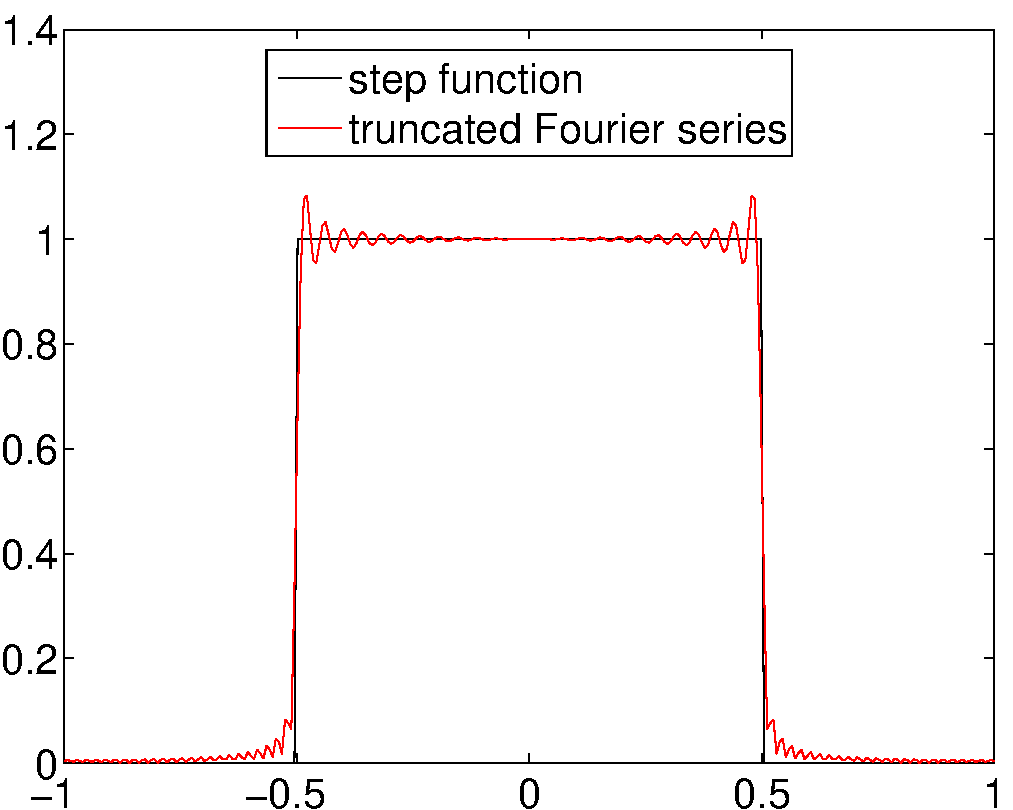
\includegraphics[width=5cm]{pics/gibbs}
  \end{center}
  \caption{Gibbs phenomenon: the overshooting of the truncated Fourier\index{Fourier!series|fig}
    series is due to the missing harmonics.}
  \label{fig:gibbs}
\end{figure}

A perfect solution to this problem is not available -- truncating the
series expansion we are wasting information that we can not
reconstruct, -- but we can formulate the eigenvalue problem so that it
is less sensible to it.

The are two possible formulations \cite{villeneuve_photonic}.
\begin{description}
\item[$\H$ formulation], which is the one described in the previous
  \secref{sec:pwe}. Helmholtz equation is written using the $\H$ field
  and discretized using plane waves, yielding the eigenproblem in
  \eqref{eqn:pwe_eigenproblem}. This formulation is usually preferred,
  because it leads to a simple eigenvalue problem, not a generalized
  one. The only difficulty is represented by the factor
  $\frac{1}{\eps}$ between the curl operators\footnote{This problem has been
  already met in \eqref{eqn:fdm_helmholtz_h}.}, that leads to the
  definition of the matrix $\Matrix{A}$. There are two
  methods to define it:
  \begin{enumerate}
  \item
    inverse expansion method: $\Matrix{A}$ is the Toeplitz\index{Toeplitz} matrix
    \cite{mathworld} obtained from the Fourier transform of
    $\frac{1}{\eps}$:
    \begin{equation*}
      \Matrix{A} = \Toeplitz \left( \Fourier{\frac{1}{\eps}} \right);
    \end{equation*}
  \item
    Ho's method \cite{ho_existence}: $\Matrix{A}$ is the inverse
    matrix of the Toeplitz matrix obtained from the Fourier transform
    of $\epsilon$:
    \begin{equation*}
      \Matrix{A} = \left(\Toeplitz \left( \Fourier{\eps} \right) \right)^{-1}.
    \end{equation*}
  \end{enumerate}
  
  Both formulations are identical in infinite-dimensional systems, but
  in truncated systems the first gives a slower convergence than the
  second. The disadvantage of the Ho's method is that taking the
  inverse of the initial (symmetric) Toeplitz matrix breaks the
  symmetry of the $\Matrix{A}$ matrix and the eigenproblem becomes a
  generalized eigenvalue problem. Interestingly enough, the Ho's
  formulation is exactly equivalent to the next $\E$ formulation.
\item[$\E$ formulation]. Helmholtz equation is written using the $\E$
  field and discretized using plane waves. Now, the matrix
  $\Matrix{A}$ is the matrix corresponding to the operator
  $\Operator{A_{\k}}{\Anything} = \CrossProd{\CrossProd{\left( \k + \Vector{G}
  \right)}{\left( \k + \Vector{G} \right)}}{\Anything}$ and the matrix
  $\Matrix{B}$ is the Toeplitz matrix obtained from the Fourier
  transform of $\epsilon$. The eigenproblem is now a generalized
  Hermitian eigenvalue problem. Compared to the $\H$ formulation, this
  leads to a faster convergence, but, even if the number of iterations
  are less, each iteration involves more floating points
  operations. Which method to use depends on the dimension of the
  whole problem and on the incident polarization.
\end{description}

This distinction closely resembles the teaching from \emph{Effective
  Medium}\index{Effective!medium} theory, about the best way of smoothing the refractive index
to improve convergence in similar eigenvalue problems: indeed,
smoothing of the refractive index is another way to alleviate the
  plane wave expansion problem, as well. There are two effective ways of smoothing
the dielectric function, depending of polarization of the incident
light, relative to the versor $\Versor{n}$ normal to the discontinuity
surface. For $\E \parallel \Versor{n}$, better results are achieved by
  averaging the inverse of
$\epsilon$; for $\E \perp \Versor{n}$, it's better to take the inverse of the
average of $\epsilon$. If the incident wave is neither TE nor TM, one
can average these two ``averages'' weighting the sum by a projection
operator $P$, that takes into account the hybrid input polarization
  \cite{johnson_block}.

This averaging method would improve convergence also in the \FDTD
algorithm, but it's never been applied there, to the Author's
knowledge: this can be due to the difficulty to define the notion of
``direction of propagation'' in an algorithm which is intrinsically
``isotropic'', in the sense that do not suppose any particular
preferred direction.

If the dielectric discontinuities have particular properties, more
effective methods than a simple smoothing can be employed
to improve convergence.

For example, if the dielectric discontinuities are piecewise constant
and parallel to the principal dielectric axes, the crystal is said to
fulfill the \emph{perpendicularity condition}
\cite{lalanne_effective}. See \figref{fig:lalanne_fig1}, for an
example of such a structure.

\begin{figure}[htbp]
  \begin{center}
    \resizebox{5cm}{!}{\input{pics/lalanne_fig1.pdf_t}}
  \end{center}
  \caption{Elementary cell of a three-dimensional square-rod
    structure, satisfying the perpendicularity condition (taken from
    \cite{lalanne_effective}).}
  \label{fig:lalanne_fig1}
\end{figure}

In this case $\E_x$ is a continuous function in $y$ and $z$ and
discontinuous in $x$. Moreover, only $\epsilon_x$ acts on $\E_x$, so
that the product $\epsilon_x \E_x$ is continuous in $x$. Therefore,
the $\E$ formulation is better employed with the $y$ and $z$
components and the $\H$ formulation is better employed with the $x$
component.

If perpendicular condition does not hold, other methods, like
\emph{super-Gaussian} functions \cite{villeneuve_photonic}, may become
competitive to smooth the dielectric discontinuities.

Finally, speed improvements are achievable thinking that, when we are
interested in studying the band diagram of a photonic crystal, we are
usually focused on the first bands, at lower frequencies: therefore,
we are only interested in the first few eigenvalues of the operator
defined in \ref{eqn:pwe_operator}. While finding all the eigenvalues
of given matrix is a very complex problem, which scales with the cube
of the dimension of the matrix ($\BigO{N^3}$), there are very efficient
algorithms to find only the first few eigenvalues, where ``first'' is
defined according to a given order relation: for example, the eigenvalues
with the lowest real part or imaginary part or modulus. In this case,
the complexity is super-linear ($\BigO{N^p}$ with $1 < p < 2$).

These algorithms are also very handy in finding the confined modes of
a defect, embedded in an almost perfect lattice. Studying a defect
with the plane expansion method is a more complicated task than
studying band structures. To define it, we need a super-cell made of
many fundamental cells of the crystal and one defect: the bigger the
super-cell, the more accurate the results. In fact, as long as the
boundary conditions in the $\PWE$ are intrinsically periodic, we are
not actually studying one defect, but an infinite number of periodic
defects in the super-cell lattice. To be confident that the results are
correct, we must take care that all the defects are decoupled,
i.e. that the super-cell is big enough. Obviously, bigger super-cells
require more plane waves in the expansion and produce many more
bands in the band diagram. Finding the resonant frequencies of the
defect can involve finding tens of modes before them, which is a
resource consuming task. It is possible, though, to reformulate the
problem \ref{eqn:pwe_operator} so that the first eigenvalues are
around a given ``target frequency'' $\omega_0$. Just let $\omega =
\omega_0 + \omega'$ and rewrite \ref{eqn:pwe_operator}:
\begin{equation} \label{eqn:pwe_operator_target} \begin{aligned}
  \Operator{A_{\k}}{\H_{\k}}  & = \frac{(\omega_0 + \omega')^2}{c^2} \H_{\k} \nonumber \\
                              & = \frac{\omega_0^2 + 2 \omega_0 \omega' + \omega'^2}{c^2} \H_{\k} \nonumber \\
  \Operator{A'_{\k}}{\H_{\k}} & = \frac{\omega'}{c^2}(\omega' + 2 \omega_0) \H_{\k},
\end{aligned} \end{equation}
with $\Operator{A'_{\k}}{\Anything} = \Operator{A_{\k}}{\Anything} -
\frac{\omega_0^2}{c^2}$. The first few eigenvalues will be around the
target frequency $\omega_0$, which can be tuned to be around the
interesting resonant frequency.

Unluckly, the operator in \ref{eqn:pwe_operator_target} has a much
smaller condition number that the one in \ref{eqn:pwe_operator},
therefore iterative methods converge more slowly: this is usually a
convenient price to pay if a good estimate of $\omega_0$ is available.

\section{Examples and Validation}

The present algorithm, as implemented by the Author, called
BandSolver from now on, has been validated by comparison with
two other programs, taken as references:
\begin{enumerate}
\item
  MPB \cite{mpb}, developed by Steven G. Johnson, based on the same
  Plane Wave Expansion algorithm;
\item
  CrystalWave \cite{crystalwave}, developed by Photon Design \cite{photond},
  based on the \FDTD algorithm.
\end{enumerate}

The validation tests are shown in \tabref{tab:validation_tests}: the
first three tests are two-dimensional photonic crystals, the last one
is a three-dimensional photonic crystal planar waveguide.

\begin{table}[htbp]
  \begin{center}
    \begin{tabular}{ccp{3cm}p{3cm}c}
      \hline
      Name & Dimension & \multicolumn{2}{c}{Description} & From \\
      \hline
      Test 1 & 2-D & Triangular lattice of rods in air & $R/\Lambda = 0.2$, $\epsilon_{sub} = 1.0$, $\epsilon_{cyl} = 12.0$ & \cite{mpb} \\
      Test 2 & 2-D & Square lattice of rods in air & $R/\Lambda = 0.2$, $\epsilon_{sub} = 1.0$, $\epsilon_{cyl} = 12.0$ & \cite{johnson_photonic} \\
      Test 3 & 2-D & Triangular lattice of holes in dielectric (line defect) & $R/\Lambda = 0.35$, $\epsilon_{sub} = 10.24$, $\epsilon_{cyl} = 1.0$ & \cite{crystalwave} \\
      Test 4 & 3-D & Triangular lattice (planar crystal waveguide) & & \cite{johnson_photonic} \\
      \hline
    \end{tabular}
  \end{center}
  \caption{Validation tests.}
  \label{tab:validation_tests}
\end{table}

For all the band diagrams, where not explicitly specified, we have the
wavevectors in abscissa and the normalized frequency, defined as $F
\eqdef f\, c/\Lambda$, in ordinate. $\Lambda$ is the lattice
constant. Error is defined as the deviation from the reference:
\begin{equation*}
  \text{Error} [\%] = \frac{F_{\text{BandSolver}} -
  F_{\text{reference}}}{F_{\text{BandSolver}}} \times 100
\end{equation*}
  
\subsubsection{Test 1}

The structure considered in this test is a two-dimensional infinite
triangular lattice of dielectric rods in air
(\figref{fig:test_1:lattice}). The lattice vectors are:
\begin{align*}
  \Vector{R}_1 = \left( \frac{\sqrt{3}}{2}, -\frac{1}{2} \right) &&
  \Vector{R}_2 = \left( \frac{\sqrt{3}}{2}, \frac{1}{2} \right)
\end{align*}
The radius of the rods is $R = 0.2 \Lambda$, their refractive index is
$n_{cyl} = \sqrt{12}$.

\figref{fig:test_1:ref} shows the reference results: the figure is
taken from \cite{mpb}. The $k$-path studied is $\Gamma-M-K-\Gamma$, in
order to scan all the possible directions of the irreducible Brillouin
zone \cite{kittel_solid}. One bandgap for the TE polarization is visible for a normalized
frequency $F$ between $0.82$ and $0.86$, while two bandgaps for the TM
polarization are visible for $0.28 < F < 0.44$ and $0.56 < F < 0.59$.

The results obtained with BandSolver are reported in
\tabref{tab:test_1}, \figref{fig:test_1:TE} and
\figref{fig:test_1:TM}, for TE and TM polarizations. We can note the
very good agreement with reference results, within $1.6\%$.

\begin{table}[htbp]
  \begin{center}
    \subtable[TE polarization.]{
    \begin{tabular}{*{5}{c}}
      \hline
      Band & k-point & $F_{\text{BandSolver}}$ & $F_{\text{MPB}}$ & Error $[\%]$ \\
      \hline
      1 & $\Gamma$ & 0 & 0 & 0 \\
        & $M$ & 0.457 & 0.46 & -0.6 \\
        & $K$ & 0.482 & 0.49 & -1.6 \\
      2 & $\Gamma$ & 0.57 & 0.565 & 0.8 \\
        & $M$ & 0.47 & 0.47 & 0 \\
        & $K$ & 0.55 & 0.55 & 0 \\
      3 & $\Gamma$ & 0.785 & 0.79 & -0.6 \\
        & $M$ & 0.68 & 0.55 & -1.4 \\
        & $K$ & 0.55 & 0.55 & 0 \\
      \hline
    \end{tabular}}
    \subtable[TM polarization.]{
    \begin{tabular}{*{5}{c}}
      \hline
      Band & k-point & $F_{\text{BandSolver}}$ & $F_{\text{MPB}}$ & Error $[\%]$ \\
      \hline
      1 & $\Gamma$ & 0 & 0 & 0 \\
        & $M$ & 0.262 & 0.26 & 0.76 \\
        & $K$ & 0.275 & 0.275 & 0 \\
      2 & $\Gamma$ & 0.563 & 0.565 & -0.36 \\
        & $M$ & 0.446 & 0.446 & 0 \\
        & $K$ & 0.49 & 0.49 & 0 \\
      3 & $\Gamma$ & 0.563 & 0.565 & -0.36 \\
        & $M$ & 0.549 & 0.55 & -0.18 \\
        & $K$ & 0.49 & 0.49 & 0 \\
      \hline
    \end{tabular}}
  \end{center}
  \caption{Test 1: TE and TM results. Note that the MPB results values have
    been extracted graphically from the available graph, so accuracy is
    not better that $0.01$. Overall accordance is within $1.6\%$.}
  \label{tab:test_1}
\end{table}

\figref{fig:test_1:real} and \figref{fig:test_1:imag} show the
$z$-component of the magnetic field of the Bloch mode for the TM
polarization at the k-point $M$, first band.

\begin{figure}[htbp]
  \begin{center}
    \subfigure[Triangular lattice. In green, the fundamental cell.]{\label{fig:test_1:lattice}\resizebox{4cm}{!}{\input{pics/test01.pdf_t}}}
    \subfigure[Reference results from \cite{mpb}.]{\label{fig:test_1:ref}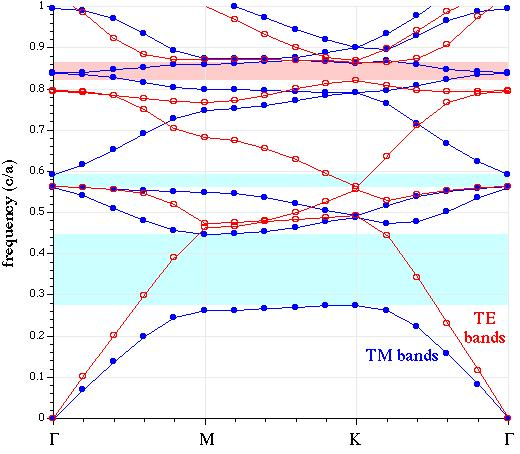
\includegraphics[width=5cm]{pics/test01_ref}}
    \subfigure[BandSolver's TE band diagram.]{\label{fig:test_1:TE}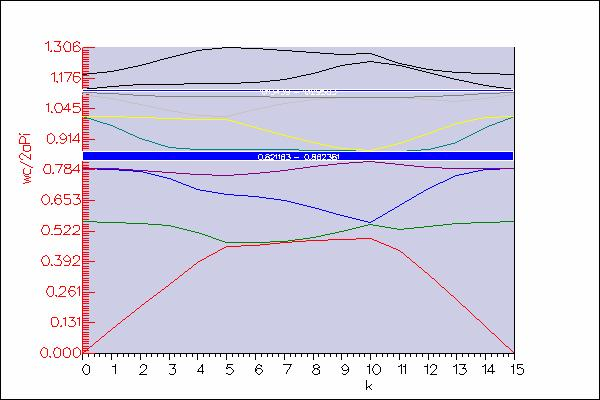
\includegraphics[width=5cm]{pics/test01_TE}}
    \subfigure[BandSolver's TM band diagram.]{\label{fig:test_1:TM}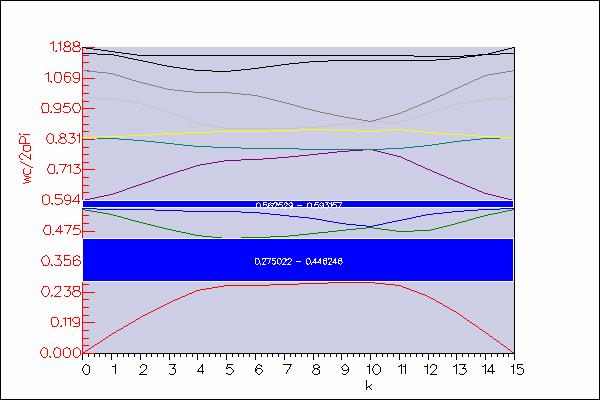
\includegraphics[width=5cm]{pics/test01_TM}}
    \subfigure[BandSolver's $\Real{H_z}$ of the Bloch mode at k-point $M$, first band]{\label{fig:test_1:real}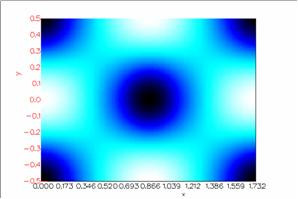
\includegraphics[width=5cm]{pics/test01_field_real}}
    \subfigure[BandSolver's $\Imag{H_z}$ of the Bloch mode at k-point $M$, first band]{\label{fig:test_1:imag}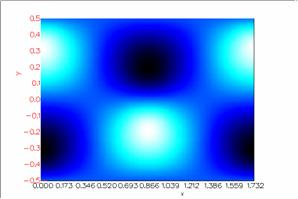
\includegraphics[width=5cm]{pics/test01_field_imag}}
  \end{center}
  \caption{Test 1.}
  \label{fig:test_1}
\end{figure}

\subsubsection{Test 2}

The structure considered in this test is a two-dimensional infinite
square lattice of dielectric rods in air
(\figref{fig:test_2:lattice}). The lattice vectors are:
\begin{equation*}
  \Vector{R}_1 = \left(1,0\right), \quad \Vector{R}_2 =
  \left(0,1\right)
\end{equation*}
The radius of the rods is $R = 0.2 \Lambda$, their refractive index is
$n_{cyl} = \sqrt{12}$.

\figref{fig:test_2:ref} shows the reference results: the figure is
taken from \cite{johnson_photonic}. The $k$-path studied is
$\Gamma-X-K-\Gamma$, in order to scan all the possible directions of
the irreducible Brillouin zone. No TE bandgaps are visible, while one
large TM bandgap is present for $0.28 < F < 0.42$.

The results obtained with our implementation are reported in
\tabref{tab:test_2}, \figref{fig:test_2:TE} and \figref{fig:test_2:TM}, for TE and TM
polarizations. We can note the very good agreement with
reference results, within $1.2\%$. The small bandgaps in the TE
polarization are not ``real'', but only the consequence of the
discretization in the k-path.

\begin{table}[htbp]
  \begin{center}
    \subtable[TE polarization.]{
    \begin{tabular}{*{5}{c}}
      \hline
      Band & k-point & $F_{\text{BandSolver}}$ & $F_{\text{MPB}}$ & Error $[\%]$ \\
      \hline
      1 & $\Gamma$ & 0 & 0 & 0 \\
        & $M$ & 0.413 & 0.42 & -0.7 \\
        & $K$ & 0.497 & 0.5 & -0.6 \\
      2 & $\Gamma$ & 0.55 & 0.565 & 1.2 \\
        & $M$ & 0.438 & 0.44 & 0.4 \\
        & $K$ & 0.586 & 0.59 & -0.7 \\
      3 & $\Gamma$ & 0.765 & 0.77 & -0.7 \\
        & $M$ & 0.636 & 0.64 & -0.6 \\
        & $K$ & 0.586 & 0.59 & -0.7 \\
      \hline
    \end{tabular}}
    \subtable[TM polarization.]{
    \begin{tabular}{*{5}{c}}
      \hline
      Band & k-point & $F_{\text{BandSolver}}$ & $F_{\text{MPB}}$ & Error $[\%]$ \\
      \hline
      1 & $\Gamma$ & 0 & 0 & 0 \\
        & $M$ & 0.243 & 0.24 & 1.2 \\
        & $K$ & 0.281 & 0.28 & 0.4 \\
      2 & $\Gamma$ & 0.551 & 0.55 & 0.2 \\
        & $M$ & 0.417 & 0.42 & -0.7 \\
        & $K$ & 0.495 & 0.50 & -1.0 \\
      3 & $\Gamma$ & 0.552 & 0.55 & 0.4 \\
        & $M$ & 0.554 & 0.555 & -0.2 \\
        & $K$ & 0.495 & 0.50 & -1.0 \\
      \hline
    \end{tabular}}
  \end{center}
  \caption{Test 2: TE and TM results. Note that the MPB results values have
    been extracted graphically from the available graph, so accuracy is
    not better that $0.01$. Overall accordance is within $1.2\%$.}
  \label{tab:test_2}
\end{table}

\figref{fig:test_2:real} and \figref{fig:test_2:imag} show the
$z$-component of the magnetic field of the Bloch mode for the TM
polarization at the k-point $X$, first band.

\begin{figure}[htbp]
  \begin{center}
    \subfigure[Square lattice. In green, the fundamental cell.]{\label{fig:test_2:lattice}\resizebox{4cm}{!}{\input{pics/test02.pdf_t}}}
    \subfigure[Reference results from \cite{johnson_photonic}.]{\label{fig:test_2:ref}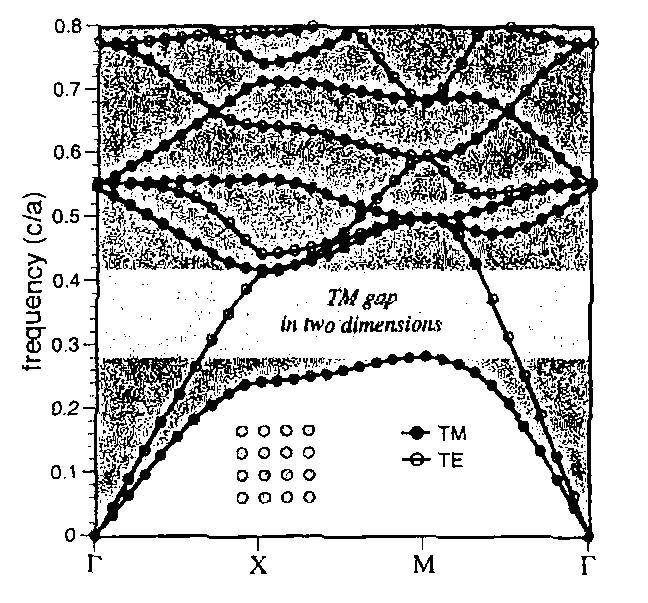
\includegraphics[width=5cm]{pics/test02_ref}}
    \subfigure[BandSolver's TE band diagram.]{\label{fig:test_2:TE}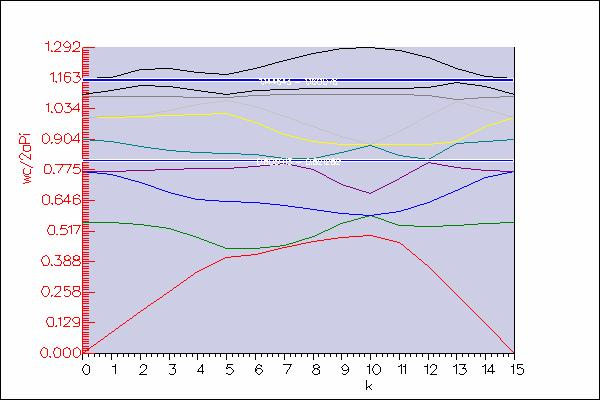
\includegraphics[width=5cm]{pics/test02_TE}}
    \subfigure[BandSolver's TM band diagram.]{\label{fig:test_2:TM}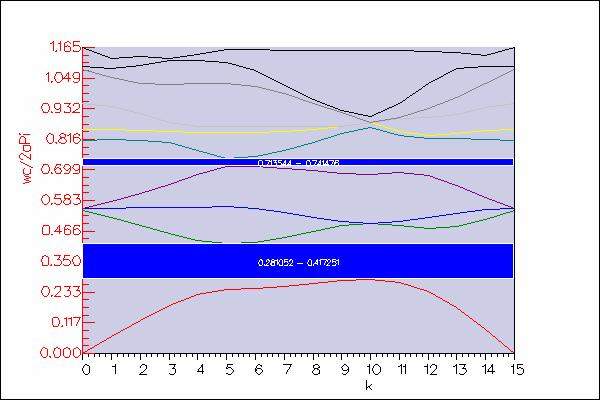
\includegraphics[width=5cm]{pics/test02_TM}}
    \subfigure[BandSolver's $\Real{H_z}$ of the Bloch mode at k-point $X$, first band]{\label{fig:test_2:real}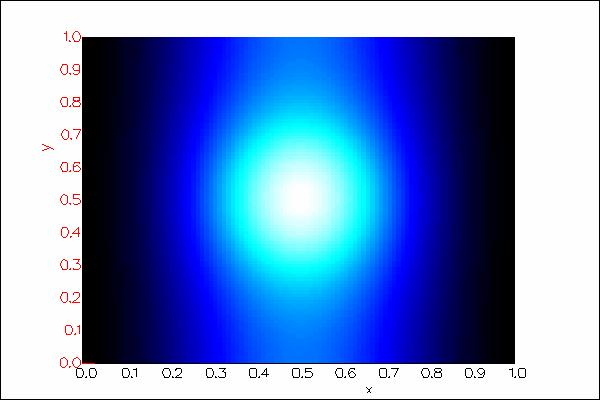
\includegraphics[width=5cm]{pics/test02_field_real}}
    \subfigure[BandSolver's $\Imag{H_z}$ of the Bloch mode at k-point $X$, first band]{\label{fig:test_2:imag}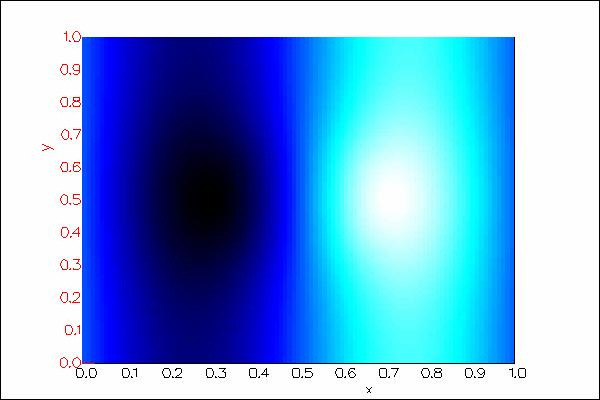
\includegraphics[width=5cm]{pics/test02_field_imag}}
  \end{center}
  \caption{Test 2.}
  \label{fig:test_2}
\end{figure}

\subsubsection{Test 3}

The structure considered in this test is a line defect in a two-dimensional 
triangular lattice of air holes in a dielectric substrate
(\figref{fig:test_3_line:lattice}). The lattice vectors are:
\begin{equation*}
  \Vector{R}_1 = \left( \frac{\sqrt{3}}{2}, -\frac{1}{2} \right),
  \quad \Vector{R}_2 = \left( \frac{\sqrt{3}}{2}, \frac{1}{2} \right)
\end{equation*}
The radius of the rods is $R = 0.309 \Lambda$, their refractive index is
$n_{sub} = 3.2$. Only the TE polarization is considered.

First, the bandgap of an infinite lattice, without defect, is
computed. Results are shown in \figref{fig:test_3:ref}, as computed by
CrystalWave, and \figref{fig:test_3:TE}, with BandSolver. Numerical
comparisons are given in \tabref{tab:test_3}.

\begin{table}[htbp]
  \begin{center}
    \begin{tabular}{*{3}{c}}
      \hline
      & First bandgap -- low $F$ & First bandgap -- high $F$ \\
      \hline
      BandSolver & 0.226 & 0.289 \\
      CrystalWave & 0.221 & 0.281 \\
      \hline
    \end{tabular}
  \end{center}
  \caption{Comparison between BandSolver and CrystalWave, on the
  boundaries of the first bandgap for the TE polarization, for the
  complete lattice. Accordance is within $2\%$.}
  \label{tab:test_3}
\end{table}

CrystalWave algorithm consists in propagating a broadband
plane wave through the crystal, collecting the result and Fourier
transforming it to get the spectral response of the device. It implicitly
studies just one direction of propagation through the crystal, the one
corresponding to the input planewave wavevector. In the example, it
corresponds to k-point $X$. This procedure is somehow limiting,
because in doesn't allow the user to study the full bandgap of the
structure: a lattice could, in fact, present a not-complete bandgap, i.e. a bandgap only for
certain directions, but non for all, and being misinterpreted for a
complete one. Our algorithm, on the other hand, scanning all the
directions of the irreducible Brillouin zone, avoids this problem and
gives a complete grasp of the device's band structure.

 \figref{fig:test_3:ref} shows the power transmitted
through the device as a function of frequency. We can note a broad
range of frequencies for which the transmission is zero: this is a
bandgap in the direction of propagation of the input planewave. It
correspond to the first bandgap (shown in blue) in
\figref{fig:test_3:TE}.

\begin{figure}[htbp]
  \begin{center}
    \subfigure[Reference results computed by CrystalWave.]{\label{fig:test_3:ref}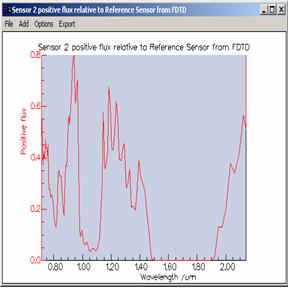
\includegraphics[width=5cm]{pics/test04_ref}}
    \subfigure[BandSolver's TE band diagram.]{\label{fig:test_3:TE}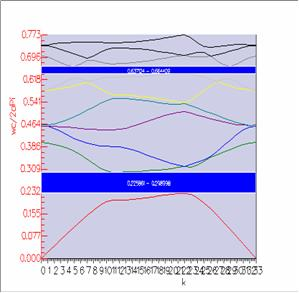
\includegraphics[width=5cm]{pics/test04_TE}}
  \end{center}
  \caption{Test 3: complete lattice.}
  \label{fig:test_3}
\end{figure}

With these informations, the line defect can now be studied. To model it, a super-cell, as shown
in \figref{fig:test_3_line:lattice} in green, is taken and only the
directions parallel to the channel's axis are studied, i.e. the
wavevectors between $\Gamma$ and $X$. The results
obtained with BandSolver are reported in
\figref{fig:test_3_line:TE}, and they have to be compared with
\figref{fig:test_3_line:ref}. Note that CrystalWave shows unitary
power for the frequencies inside the bandgap: they are guided
lossless by the line defect through the crystal. The small deep at
the middle of the bandgap corresponds to the crossing point between
the even guided mode (whose characteristic has negative slope) and the
odd mode (whose characteristic has positive slope) in
\figref{fig:test_3_line:TE}. It is due to the fact that, for that
particular wavevector, the phase
velocity of the excited mode (which is the even mode, in CrystalWave)
is almost zero (i.e., its characteristic is almost flat): in a time-domain
algorithm as CrystalWave's, this means that power takes very long time to
get to the end of the device and to be computed in the \FFT. Lasting the
simulation longer would reduce the deep.

\begin{figure}[htbp]
  \begin{center}
    \subfigure[Line defect. In green, the super-cell.]{\label{fig:test_3_line:lattice}\resizebox{8cm}{!}{\input{pics/test04.pdf_t}}}
    \subfigure[Reference results computed by CrystalWave.]{\label{fig:test_3_line:ref}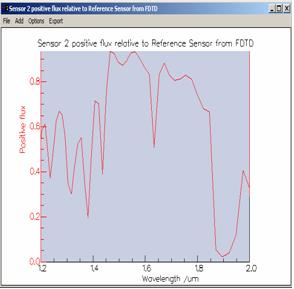
\includegraphics[width=5cm]{pics/test04_line_ref}}
    \subfigure[BandSolver's TE band diagram.]{\label{fig:test_3_line:TE}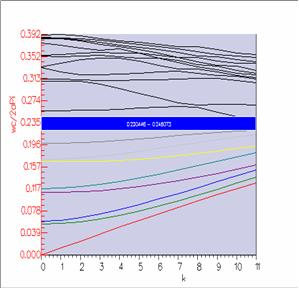
\includegraphics[width=5cm]{pics/test04_line_TE}}
    \subfigure[BandSolver's Real $H_z$.]{\label{fig:test_3_line:real}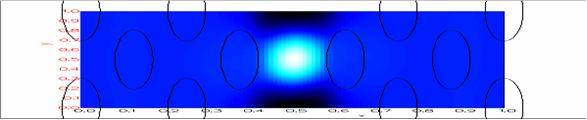
\includegraphics[width=5cm]{pics/test04_line_field_real}}
    \subfigure[BandSolver's Imag $H_z$.]{\label{fig:test_3_line:imag}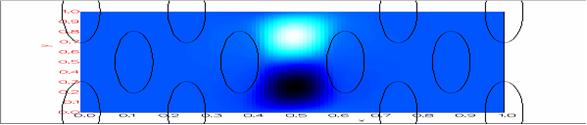
\includegraphics[width=5cm]{pics/test04_line_field_imag}}
  \end{center}
  \caption{Test 3: line defect.}
  \label{fig:test_3_line}
\end{figure}

The $z$-component of the magnetic field of the fundamental guided mode
in the super-cell is shown in \figref{fig:test_3_line:real} and
\figref{fig:test_3_line:imag}.

\subsubsection{Test 4}

The structure considered in this test is a planar photonic crystal
waveguide, made of a triangular lattice of dielectric rods in air,
refractive index $n_{cil}^{high} = 3$, height $H = \Lambda$,
and refractive index $n_{cil}^{low} = 2$ infinitely above and below, radius
$R = 0.3 \Lambda$. See \figref{fig:test_4}.

\begin{figure}[htbp]
  \begin{center}
    \subfigure[Triangular lattice from \cite{johnson_photonic}.]{\label{fig:test_4:lattice}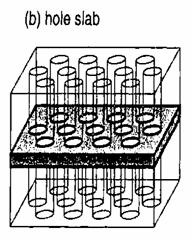
\includegraphics[width=5cm]{pics/test06}}\\
    \subfigure[Reference results from \cite{johnson_photonic}.]{\label{fig:test_4:ref}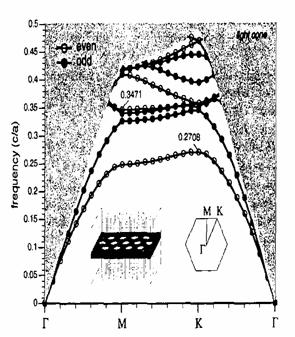
\includegraphics[height=5cm,width=5.5cm]{pics/test06_ref}}
    \subfigure[BandSolver's band diagram.]{\label{fig:test_4:bands}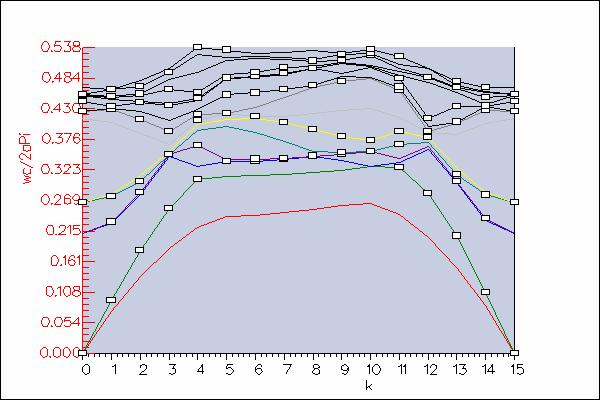
\includegraphics[height=5cm,width=6cm]{pics/test06_bands}}
  \end{center}
  \caption{Test 4.}
  \label{fig:test_4}
\end{figure}

\figref{fig:test_4:ref} shows the reference results and
\figref{fig:test_4:bands} the computed ones: \tabref{tab:test_4} shows
that the accordance is again very good.

\begin{table}[htbp]
  \begin{center}
    \begin{tabular}{*{5}{c}}
      \hline
      Band & k-point & $F_{\text{our algorithm}}$ & $F_{\text{MPB}}$ & Error $[\%]$ \\
      \hline
      1 & $\Gamma$ & 0 & 0 & 0 \\
        & $M$ & 0.237 & 0.24 & -1.3 \\
        & $K$ & 0.268 & 0.27 & -0.7 \\
      2 & $\Gamma$ & 0 & 0 & 0 \\
        & $M$ & 0.312 & 0.32 & 2.6 \\
        & $K$ & 0.328 & 0.34 & -3.7 \\
      3 & $\Gamma$ & 0.215 & n/a & n/a \\
        & $M$ & 0.328 & 0.34 & -3.7 \\
        & $K$ & 0.328 & 0.34 & -3.7 \\
      \hline
    \end{tabular}
  \end{center}
  \caption{Test 4: comparison between the reference results and our
  algorithm's result. Overall accordance is within $3.7\%$.}
  \label{tab:test_4}
\end{table}

As an example, \figref{fig:test_4_field} shows the profile of the real
part of the Bloch mode at the reciprocal lattice point $M$, first
band. The fields are plotted on an horizontal section passing through
the high index slab and on a vertical section passing through the
center of a unit cell.

\begin{figure}[htbp]
  \begin{center}
    \subfigure[Horizontal section, $x$ component]{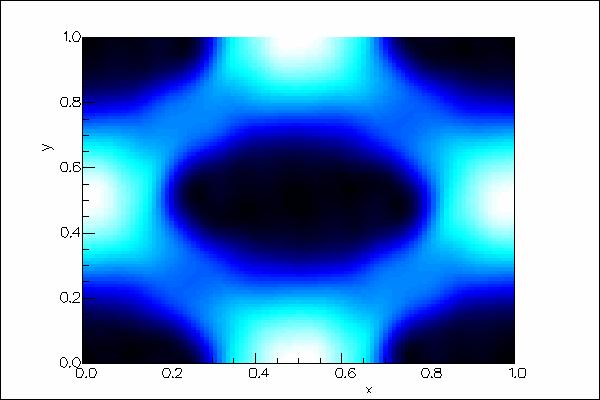
\includegraphics[width=5cm]{pics/test06_field_hor_x}}
    \subfigure[Horizontal section, $y$ component]{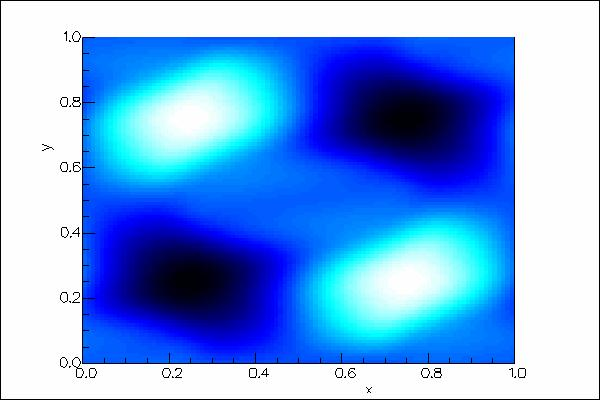
\includegraphics[width=5cm]{pics/test06_field_hor_y}}
    \subfigure[Vertical section, $x$ component]{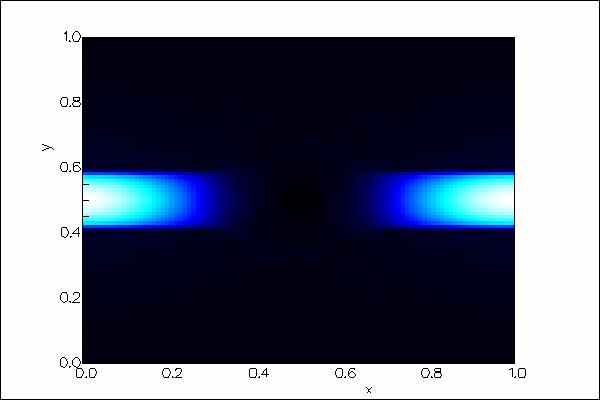
\includegraphics[width=5cm]{pics/test06_field_ver_x}}
    \subfigure[Vertical section, $y$ component]{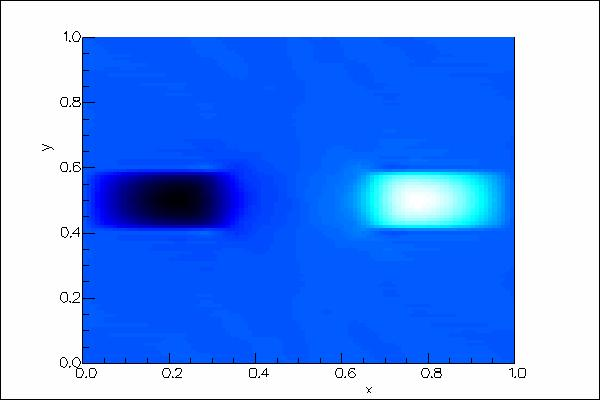
\includegraphics[width=5cm]{pics/test06_field_ver_y}}
  \end{center}
  \caption{Test 4: Real part of the Bloch mode, at k-point $M$, first
  band, computed by BandSolver. Values on the axis are normalized to
  the lattice constant $\Lambda$.}
  \label{fig:test_4_field}
\end{figure}

\vspace{2cm}
A commercial implementation of BandSolver is available from Photon Design \cite{photond}.

\index{Plane Wave Expansion|)}

%% \OKKIO{
%%   photonic crystals:
%% \begin{enumerate}
%% \item
%%   introduction: what are they -> see my thesis
%% \item
%%   XXX how do you describe them: crystal lattices, reciprocal lattice
%% \item
%%   how do you study them analitycally: yeh yariv electromagnetic -> theory
%% \item
%%   what can you do with them:
%%   \begin{enumerate}
%%     \item
%%       broeng photonic, maradudin out of plane -> photonic crystal
%%       fibers
%%     \item
%%       boscolo superprism, enoch numerical -> superprism -> NIM
%%   \end{enumerate}
%% \end{enumerate}
%% }

